In this document we present some of the samples from the various GAN setups in full page figures below.

We also note that the GAN approach to density estimation is complementary to the earlier \emph{density ratio estimation} approach~\citep{Sugiyama2012}\@.
In density ratio estimation, the generator $G$ is fixed, and the density is found by combining Bayes' rule and the learned classifier $D$.
In GANs, the key is learning $G$ well; while in density ratio estimation, the key is learning $D$ well.
The MH-GAN has flavors of both in that it uses both $G$ and $D$ to build $G'$.

\begin{figure*}[htbp]
    \centering
    \includegraphics[width=\exfactor\textwidth]{figures/pgan/all_base_iso_base_lq.jpg}
    \caption{
    Set of 64 random samples from the (base) PGAN\@.
    }
\end{figure*}

\begin{figure*}[htbp]
    \centering
       
\includegraphics[width=0.2\textwidth]{figures/pgan/4_base_iso_base.jpg}
    \hfill
       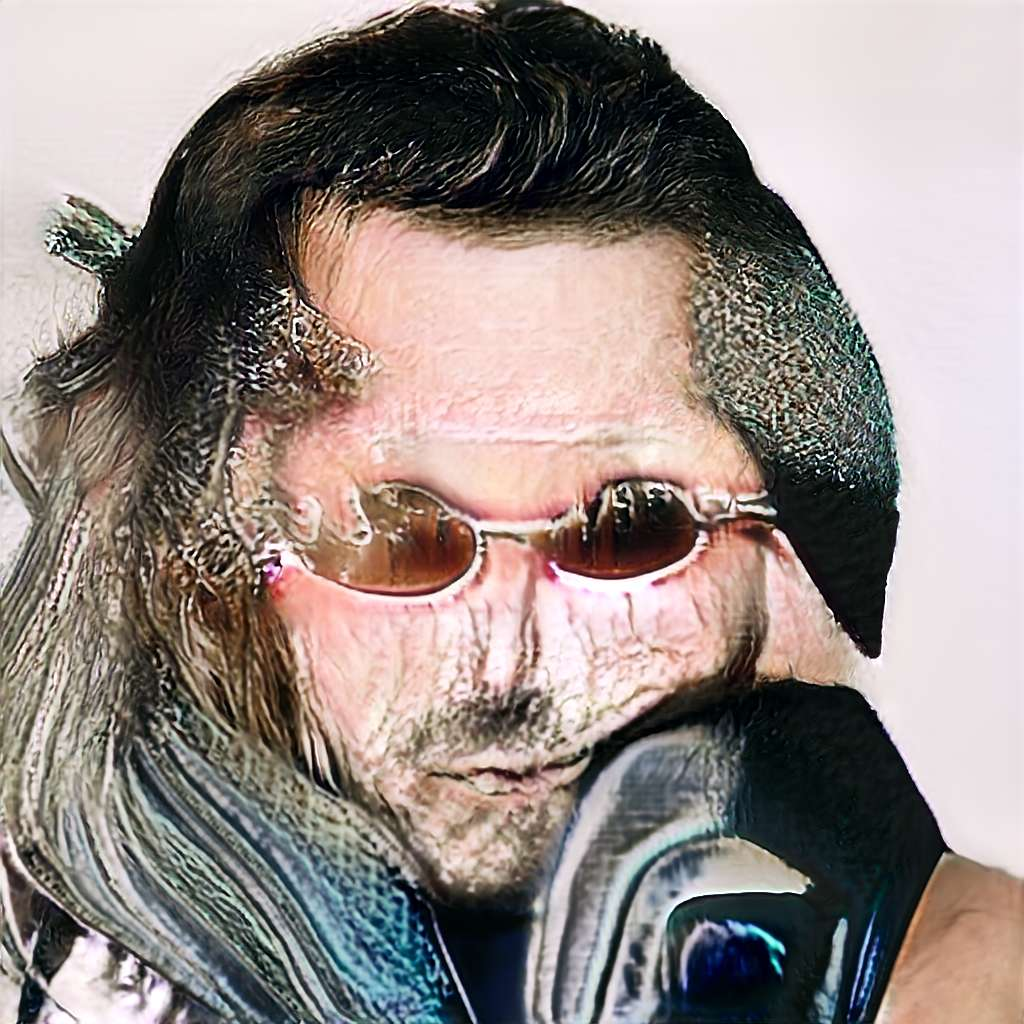
\includegraphics[width=0.2\textwidth]{figures/pgan/5_base_iso_base.jpg}
    \hfill
       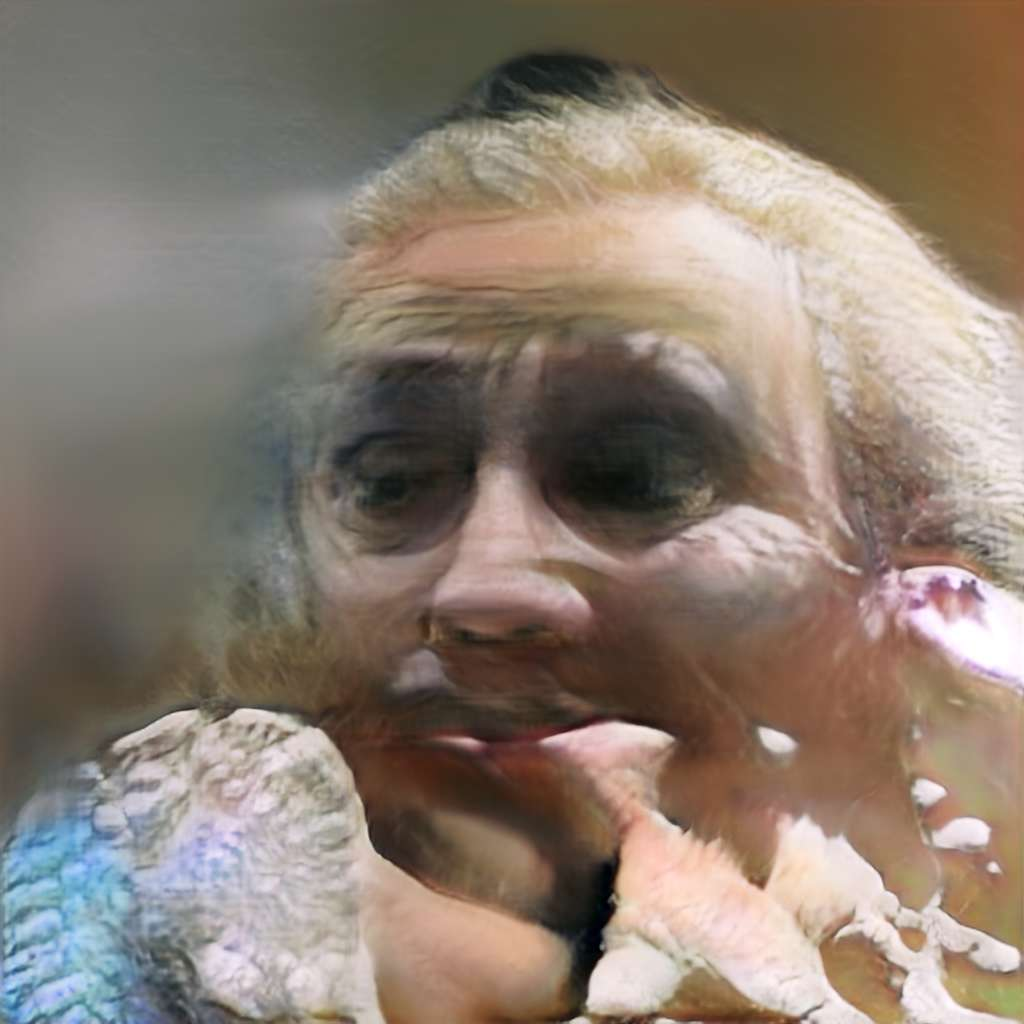
\includegraphics[width=0.2\textwidth]{figures/pgan/8_base_iso_base.jpg}
    \hfill
       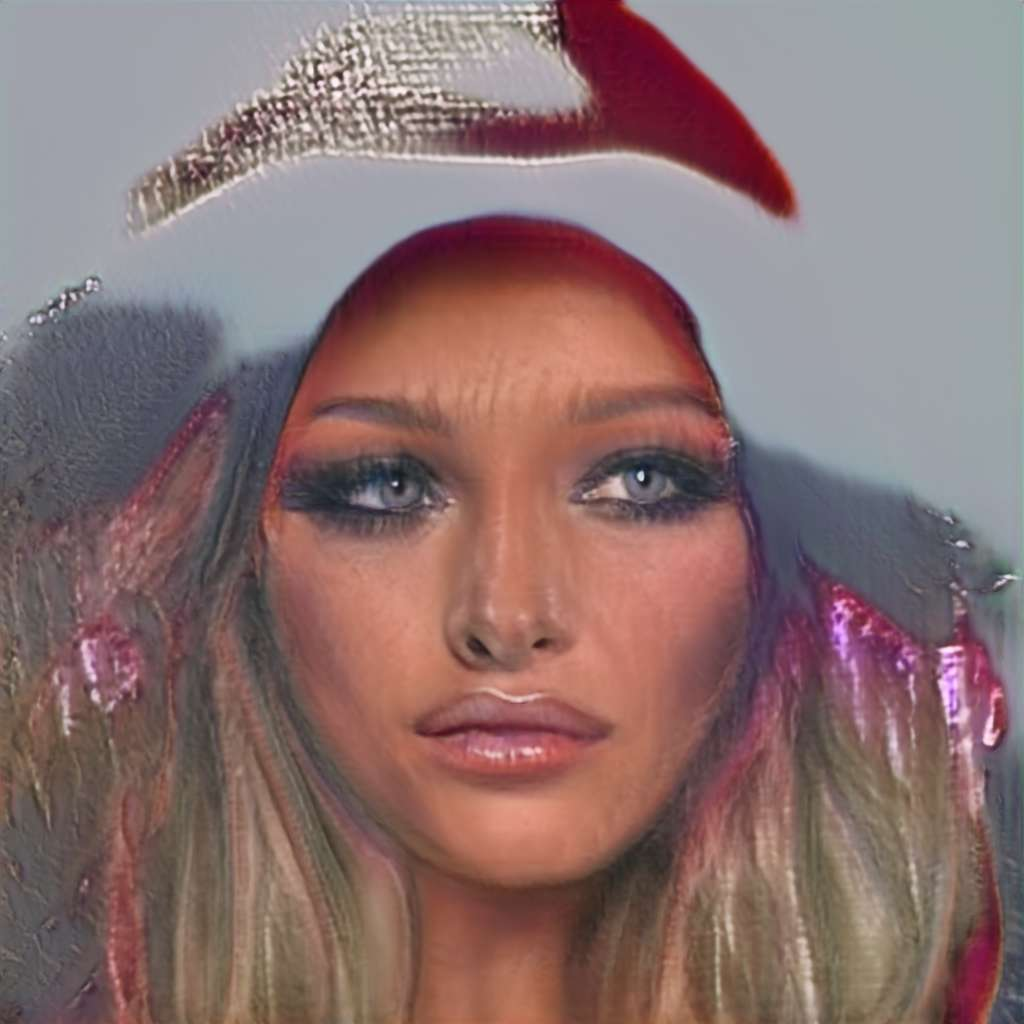
\includegraphics[width=0.2\textwidth]{figures/pgan/34_base_iso_base.jpg}
    \caption{
    Flawed examples from the PGAN\@.
    Such a degree of non-realism is rarer in the DRS samples (Figure~\ref{fig:DRS 64x}) and nearly absent in the MH-GAN samples (Figure~\ref{fig:MHGAN 64x})\@.
    }
\end{figure*}

\begin{figure*}[htbp]
    \centering
    \includegraphics[width=\exfactor\textwidth]{figures/pgan/all_base_iso_reject_lq.jpg}
    \caption{
    Set of 64 random samples from the calibrated DRS setup.
    }
    \label{fig:DRS 64x}
\end{figure*}

\begin{figure*}[htbp]
    \centering
    \includegraphics[width=\exfactor\textwidth]{figures/pgan/all_base_iso_MH_lq.jpg}
    \caption{
    Set of 64 random samples from the calibrated MH-GAN\@.
    }
    \label{fig:MHGAN 64x}
\end{figure*}

\begin{figure}[htbp]
    \centering
    \begin{subfigure}[b]{0.49\textwidth}
       \centering
       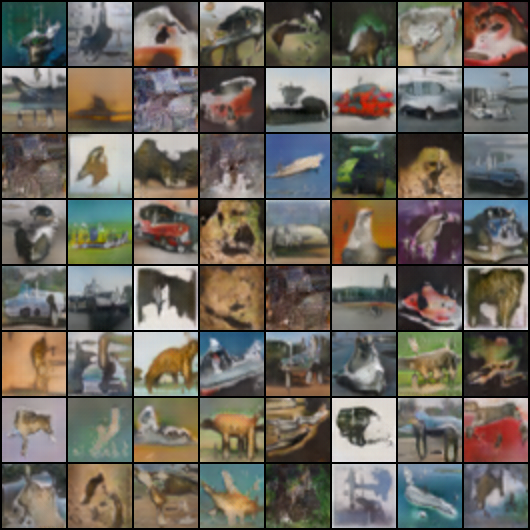
\includegraphics[width=1.0\textwidth]{figures/cifar/192_base_raw_base.png}
       \caption{GAN}
    \end{subfigure}
    \begin{subfigure}[b]{0.49\textwidth}
       \centering
       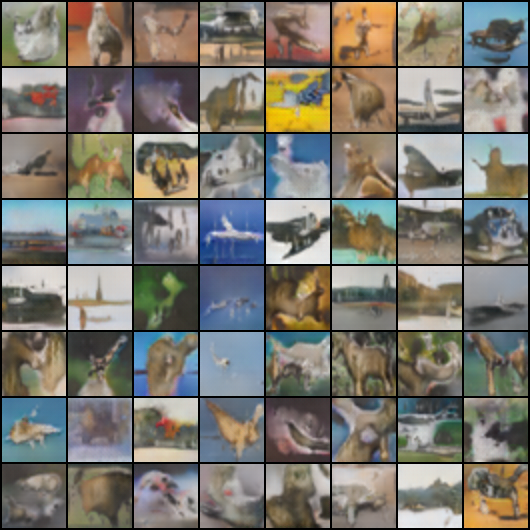
\includegraphics[width=1.0\textwidth]{figures/cifar/192_base_raw_reject.png}
       \caption{DRS}
    \end{subfigure}
    \begin{subfigure}[b]{0.49\textwidth}
       \centering
       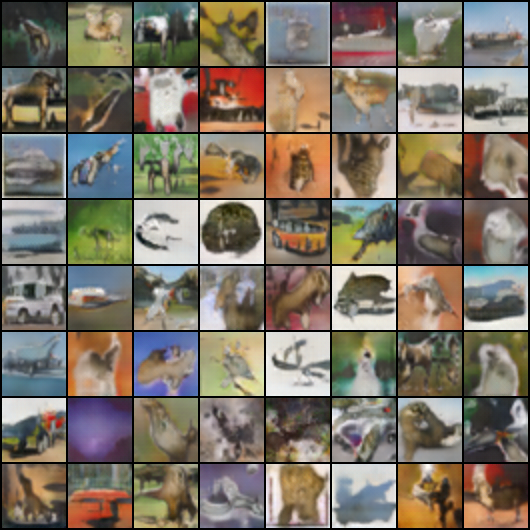
\includegraphics[width=1.0\textwidth]{figures/cifar/192_base_raw_MH.png}
       \caption{MH-GAN}
    \end{subfigure}
    \begin{subfigure}[b]{0.49\textwidth}
       \centering
       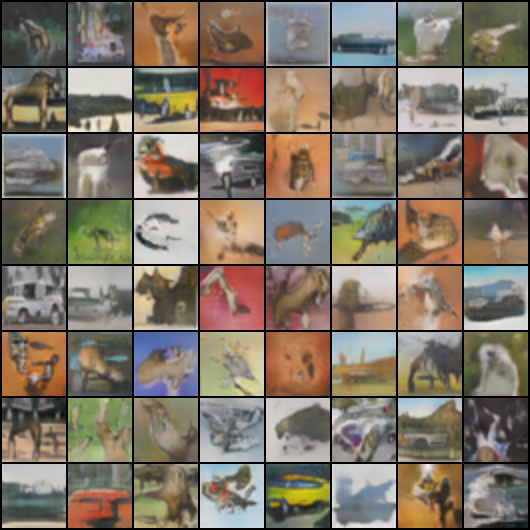
\includegraphics[width=1.0\textwidth]{figures/cifar/192_base_iso_MH.png}
       \caption{MH-GAN (cal)}
    \end{subfigure}
    \caption{{\small
    Example images on CIFAR-10 for different GAN setups.
    The different selectors (MH-GAN and DRS) are run on the same batch of images.
    Meaning, the same images may appear for both generators.
    The calibrated MH-GAN shows a greater preference for animal-like images with four legs.
    }}
    \label{fig:cifar_samples}
\end{figure}


\begin{figure}[htbp]
    \centering
    \begin{subfigure}[b]{0.49\textwidth}
       \centering
       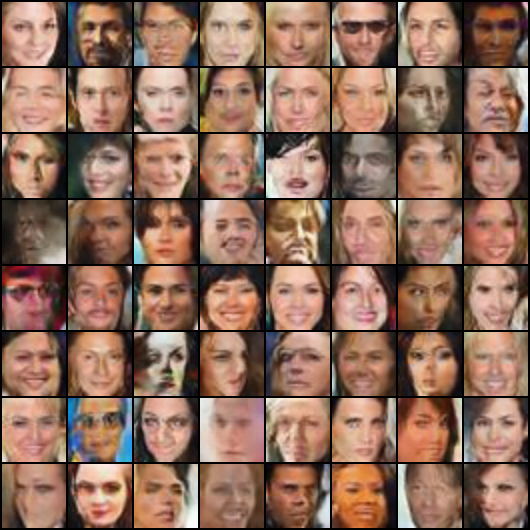
\includegraphics[width=\exfactor\textwidth]{figures/celeba/31_base_raw_base.png}
       \caption{GAN}
    \end{subfigure}
    \begin{subfigure}[b]{0.49\textwidth}
       \centering
       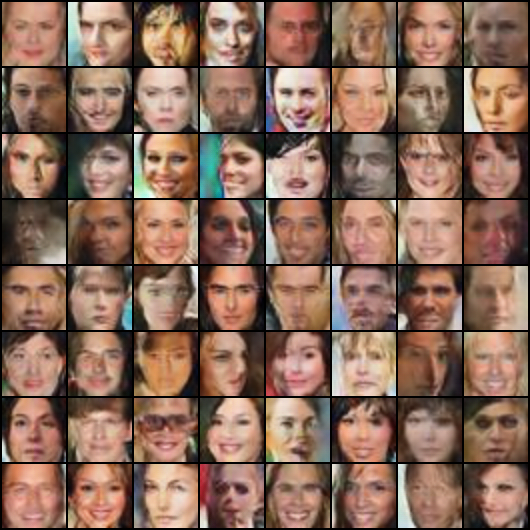
\includegraphics[width=\exfactor\textwidth]{figures/celeba/31_base_raw_reject.png}
       \caption{DRS}
    \end{subfigure}
    \begin{subfigure}[b]{0.49\textwidth}
       \centering
       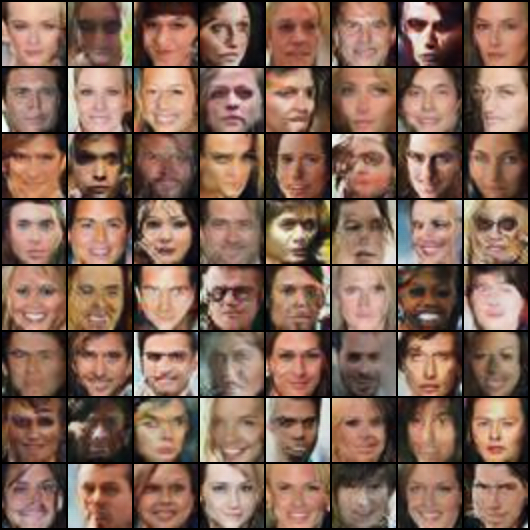
\includegraphics[width=\exfactor\textwidth]{figures/celeba/31_base_raw_MH.png}
       \caption{MH-GAN}
    \end{subfigure}
    \begin{subfigure}[b]{0.49\textwidth}
       \centering
       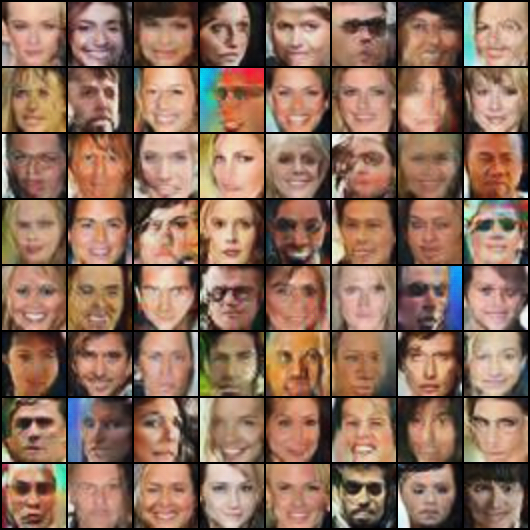
\includegraphics[width=\exfactor\textwidth]{figures/celeba/31_base_iso_MH.png}
       \caption{MH-GAN (cal)}
    \end{subfigure}
    \caption{{\small
    Example images on CelebA for different GAN setups.
    Like Figure~\ref{fig:cifar_samples}, the same batch of images goes into each selector.
    }}
    \label{fig:celeba_samples}
\end{figure}


